%---------------------------------------------------------------------
%
%                          Ap�ndice 1
%
%---------------------------------------------------------------------

\chapter{Schematics}
\label{ap1:schematics}

%\topskip0pt
\vspace*{\fill}

\begin{figure}[!h]
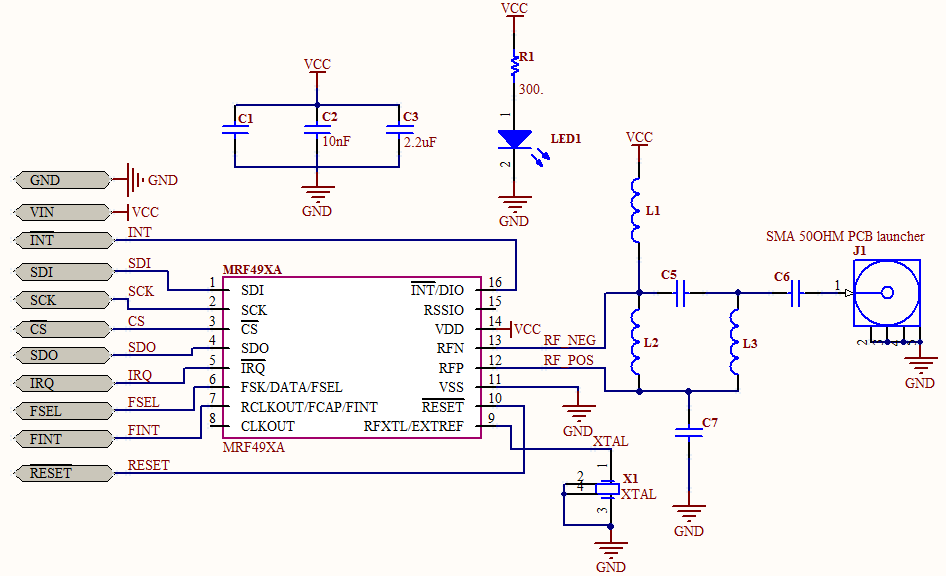
\includegraphics[width=.9\textwidth]{Imagenes/Bitmap/Apendices/mtransschematic}
\caption{$\mu$Trans 434/868 schematic.}
\label{ap1:mtransschematic}
\end{figure}

\begin{table}[!h]
\centering
\scalebox{0.8}{
\begin{tabular}{||c|c|c|c|c|c|c|c||}
\hline
Freq & C1 & L1 & L2 & L3 & C5 & C6 & C7 \\ \hline  \hline
434 MHz & 220 pF & 390 nH & 33 nH & 47 nH & 2.7pF & 68 pF & 5.1 pF \\ \hline
868 MHz & 47 pF & 100 nH & 8.2 nH & 22 nH & 1.2 pF & 27 pF & 2.7 pF \\ \hline
\end{tabular}}
\caption{Values for balun components at different frequency bands.
\label{tab:cap4:balunvalues}}
\end{table}

\vspace*{\fill}

\newpage\null\thispagestyle{empty}\newpage

\vspace*{\fill}

\begin{figure}[!h]
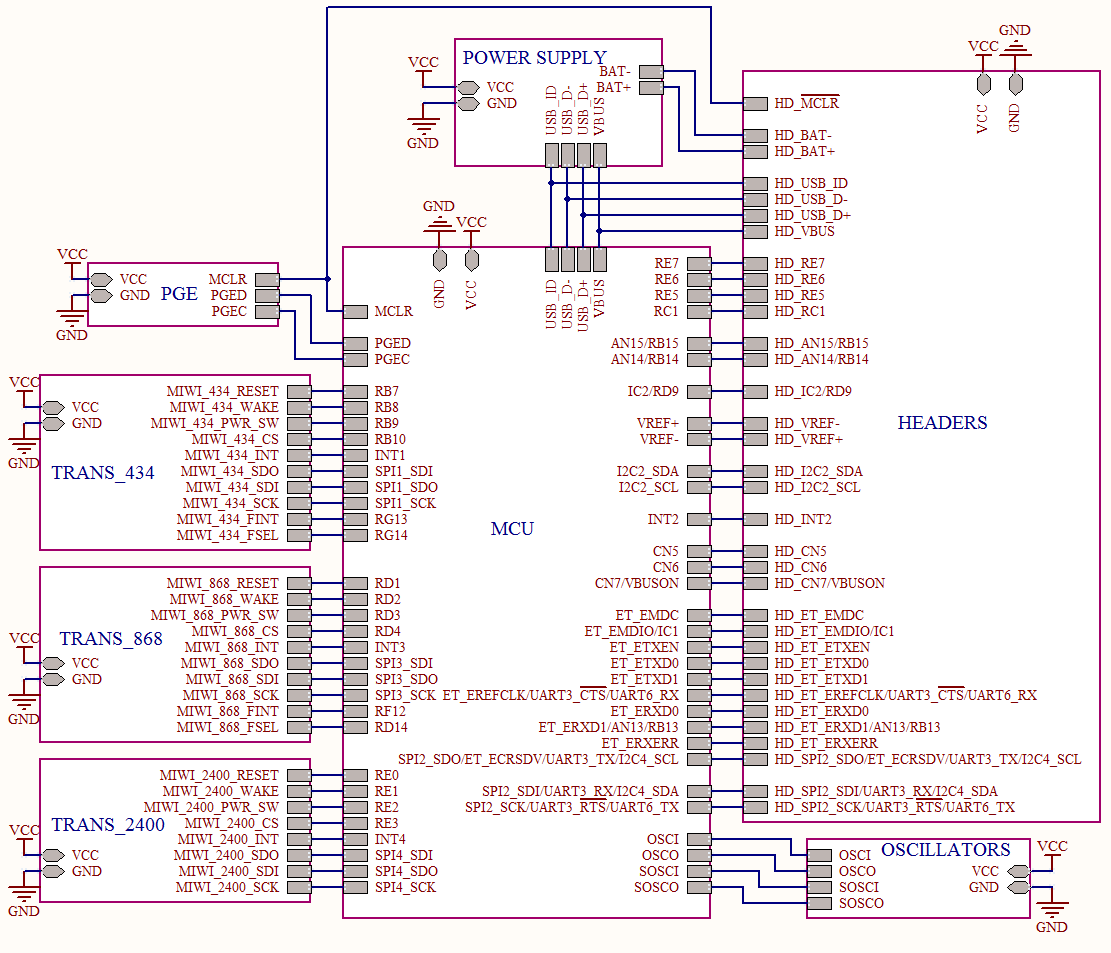
\includegraphics[width=1.1\textwidth]{Imagenes/Bitmap/Apendices/schematic}
\caption{cNGD general schematic.}
\label{fig:cap4:gneralschematic}
\end{figure}

\vspace*{\fill}

\newpage\null\thispagestyle{empty}\newpage

\vspace*{\fill}

\begin{figure}[!h]
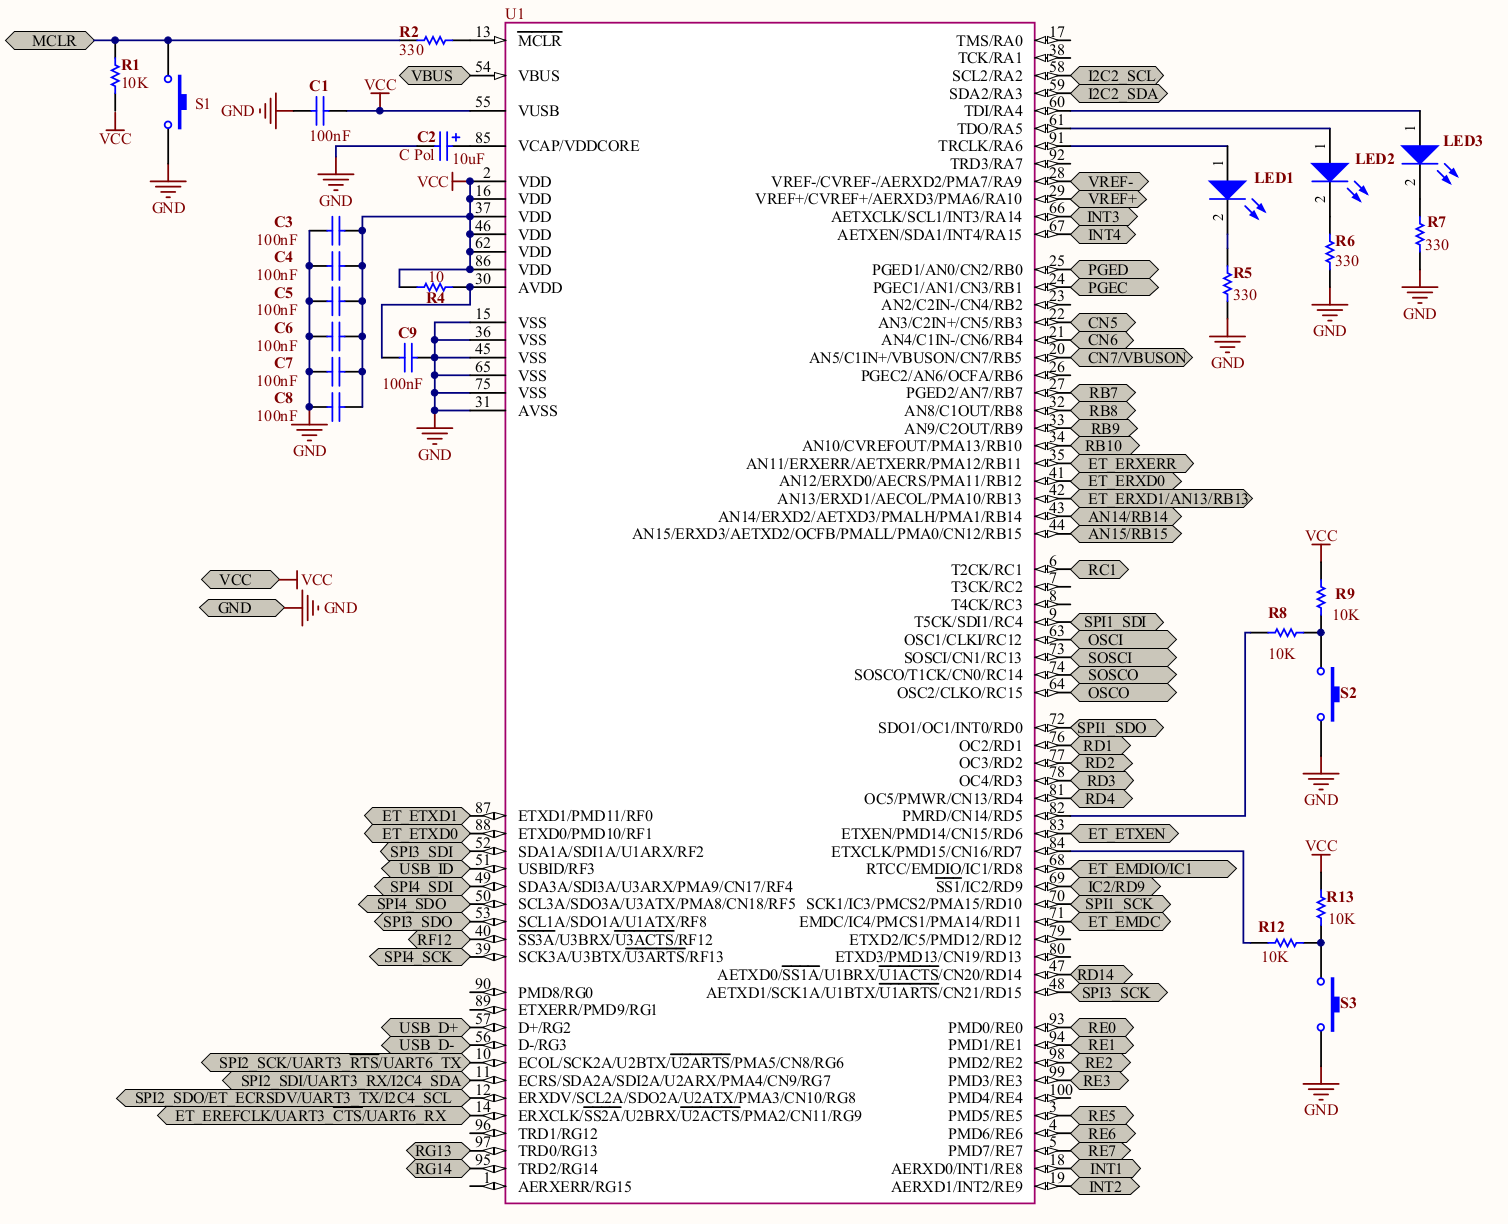
\includegraphics[width=1.1\textwidth]{Imagenes/Bitmap/Apendices/MCU}
\caption{Microcontroller specific schematic.}
\label{fig:cap4:mcuschematics}
\end{figure}

\vspace*{\fill}

\newpage\null\thispagestyle{empty}\newpage

\vspace*{\fill}

\figura{Bitmap/Apendices/434}{width=0.8\textwidth}{fig:cap4:434schematics}%
{434 MHz Radio Interface systems schematic.}

\figura{Bitmap/Apendices/868}{width=0.8\textwidth}{fig:cap4:868schematics}%
{868 MHz Radio Interface systems schematic.}

\vspace*{\fill}

\newpage\null\thispagestyle{empty}\newpage

\vspace*{\fill}

\figura{Bitmap/Apendices/2_4}{width=0.8\textwidth}{fig:cap4:2.4schematics}%
{2.4 GHz Radio Interface systems schematic.}

\figura{Bitmap/Apendices/powersupply}{width=1\textwidth}{fig:cap4:powersupplyschematic}%
{Power supply system schematic.}

\vspace*{\fill}

\newpage\null\thispagestyle{empty}\newpage

\vspace*{\fill}

\figura{Bitmap/Apendices/headers}{width=1.1\textwidth}{fig:cap4:headerschematic}%
{Expansion header system schematic.}

\figura{Bitmap/Apendices/oscillatorschematic}{width=0.5\textwidth}{fig:cap4:oscillatorschematic}%
{Oscillator system schematic.}

\figura{Bitmap/Apendices/pgeschematic}{width=0.5\textwidth}{fig:cap4:pgeschematic}%
{PGE system schematic.}

\vspace*{\fill}

\newpage\null\thispagestyle{empty}\newpage

\vspace*{\fill}

\figura{Bitmap/Apendices/rs232shieldshematic}{width=.8\textwidth}{fig:cap4:rs232shieldschematic}%
{rs232SHIELD schematic.}

\figura{Bitmap/Apendices/chargerschematic}{width=.8\textwidth}{fig:cap4:chargershematic}%
{chargerSHIELD schematic.}

\vspace*{\fill}

% Variable local para emacs, para  que encuentre el fichero maestro de
% compilaci�n y funcionen mejor algunas teclas r�pidas de AucTeX
%%%
%%% Local Variables:
%%% mode: latex
%%% TeX-master: "../Tesis.tex"
%%% End:
